\section{Results}
\label{sec:res}


\begin{figure}[h]
    \begin{tikzpicture}
        \begin{axis}[legend pos=south east]
            \addplot table [x=fall-out, y=recall, col sep=comma]
            {../analysis/generated_patients_all_no_freq_res_ROC.analysis};
            \addlegendentry{no freq}

            \addplot table [x=fall-out, y=recall, col sep=comma]
            {../analysis/generated_patients_all_k_res_ROC.analysis};
            \addlegendentry{$k$-least freq}
            
            \addplot table [x=fall-out, y=recall, col sep=comma]
            {../analysis/generated_patients_all_sampling_res_ROC.analysis};
            \addlegendentry{sampling}
            
            \addplot table [x=fall-out, y=recall, col sep=comma]
            {../analysis/generated_patients_all_p_sampling_res_ROC.analysis};
            \addlegendentry{$p$-sampling}

            \addplot table [x=fall-out, y=recall, col sep=comma]
            {../analysis/generated_patients_all_ic_res_ROC.analysis};
            \addlegendentry{IC-sampling}
        \end{axis}
    \end{tikzpicture}
    \caption{ROC curve for artificial patients infected with a general disease.}
\end{figure}

\begin{figure}[h]
    \begin{tikzpicture}
        \begin{axis}[legend pos=south east]
            \addplot table [x=fall-out, y=recall, col sep=comma]
            {../analysis/generated_patients_neg_no_freq_res_ROC.analysis};
            \addlegendentry{no freq}

            \addplot table [x=fall-out, y=recall, col sep=comma]
            {../analysis/generated_patients_neg_k_res_ROC.analysis};
            \addlegendentry{$k$-least freq}
            
            \addplot table [x=fall-out, y=recall, col sep=comma]
            {../analysis/generated_patients_neg_sampling_res_ROC.analysis};
            \addlegendentry{sampling}
            
            \addplot table [x=fall-out, y=recall, col sep=comma]
            {../analysis/generated_patients_neg_p_sampling_res_ROC.analysis};
            \addlegendentry{$p$-sampling}
            
            \addplot table [x=fall-out, y=recall, col sep=comma]
            {../analysis/generated_patients_neg_ic_res_ROC.analysis};
            \addlegendentry{IC-sampling}
        \end{axis}
    \end{tikzpicture}
    \caption{ROC curve for artificial patients infected with a
        negatively-annotated disease.}
\end{figure}

\begin{figure}[h]
    \begin{tikzpicture}
        \begin{axis}[legend pos=south east]
            \addplot table [x=fall-out, y=recall, col sep=comma]
            {../analysis/phenotips_no_freq_res_ROC.analysis};
            \addlegendentry{no freq}

            \addplot table [x=fall-out, y=recall, col sep=comma]
            {../analysis/phenotips_k_res_ROC.analysis};
            \addlegendentry{$k$-least freq}
            
            \addplot table [x=fall-out, y=recall, col sep=comma]
            {../analysis/phenotips_sampling_res_ROC.analysis};
            \addlegendentry{sampling}
            
            \addplot table [x=fall-out, y=recall, col sep=comma]
            {../analysis/phenotips_p_sampling_res_ROC.analysis};
            \addlegendentry{$p$-sampling}

            \addplot table [x=fall-out, y=recall, col sep=comma]
            {../analysis/phenotips_ic_res_ROC.analysis};
            \addlegendentry{IC-sampling}
        \end{axis}
    \end{tikzpicture}
    \caption{ROC curve for naturalistic patients.}
\end{figure}


\begin{figure}[h]
    \begin{tikzpicture}
        \begin{axis}
            \addplot table [y=precision, x=recall, col sep=comma]
            {../analysis/generated_patients_all_no_freq_res_PR.analysis};
            \addlegendentry{no freq}

            \addplot table [y=precision, x=recall, col sep=comma]
            {../analysis/generated_patients_all_k_res_PR.analysis};
            \addlegendentry{$k$-least freq}
            
            \addplot table [y=precision, x=recall, col sep=comma]
            {../analysis/generated_patients_all_sampling_res_PR.analysis};
            \addlegendentry{sampling}
            
            \addplot table [y=precision, x=recall, col sep=comma]
            {../analysis/generated_patients_all_p_sampling_res_PR.analysis};
            \addlegendentry{$p$-sampling}
            
            \addplot table [y=precision, x=recall, col sep=comma]
            {../analysis/generated_patients_all_ic_res_PR.analysis};
            \addlegendentry{IC-sampling}
        \end{axis}
    \end{tikzpicture}
    \caption{Precision-recall curve for artificial patients infected with a general disease.}
\end{figure}

\begin{figure}[h]
    \begin{tikzpicture}
        \begin{axis}
            \addplot table [y=precision, x=recall, col sep=comma]
            {../analysis/generated_patients_neg_no_freq_res_PR.analysis};
            \addlegendentry{no freq}

            \addplot table [y=precision, x=recall, col sep=comma]
            {../analysis/generated_patients_neg_k_res_PR.analysis};
            \addlegendentry{$k$-least freq}
            
            \addplot table [y=precision, x=recall, col sep=comma]
            {../analysis/generated_patients_neg_sampling_res_PR.analysis};
            \addlegendentry{sampling}
            
            \addplot table [y=precision, x=recall, col sep=comma]
            {../analysis/generated_patients_neg_p_sampling_res_PR.analysis};
            \addlegendentry{$p$-sampling}
            
            \addplot table [y=precision, x=recall, col sep=comma]
            {../analysis/generated_patients_neg_ic_res_PR.analysis};
            \addlegendentry{IC-sampling}
        \end{axis}
    \end{tikzpicture}
    \caption{Precision-recall curve for artificial patients infected with a
    negatively-annotated disease.}
\end{figure}

\begin{figure}[h]
    \begin{tikzpicture}
        \begin{axis}
            \addplot table [y=precision, x=recall, col sep=comma]
            {../analysis/phenotips_no_freq_res_PR.analysis};
            \addlegendentry{no freq}

            \addplot table [y=precision, x=recall, col sep=comma]
            {../analysis/phenotips_k_res_PR.analysis};
            \addlegendentry{$k$-least freq}
            
            \addplot table [y=precision, x=recall, col sep=comma]
            {../analysis/phenotips_sampling_res_PR.analysis};
            \addlegendentry{sampling}
            
            \addplot table [y=precision, x=recall, col sep=comma]
            {../analysis/phenotips_p_sampling_res_PR.analysis};
            \addlegendentry{$p$-sampling}
            
            \addplot table [y=precision, x=recall, col sep=comma]
            {../analysis/phenotips_ic_res_PR.analysis};
            \addlegendentry{IC-sampling}
        \end{axis}
    \end{tikzpicture}
    \caption{Precision-recall curve for naturalistic patients.}
\end{figure}


\begin{figure}[h]
    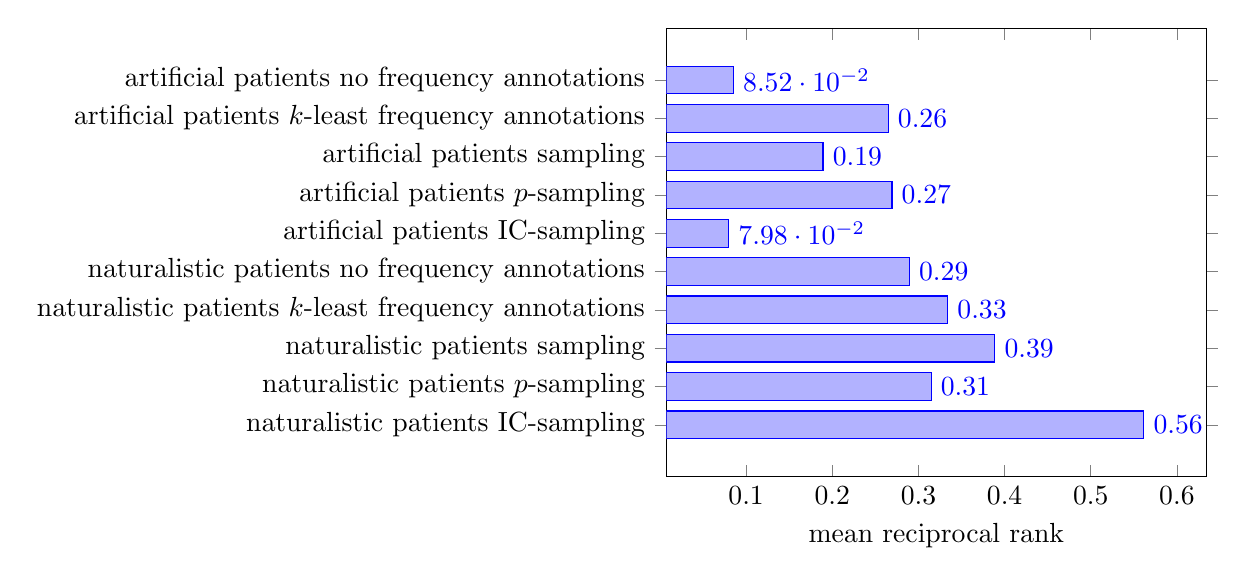
\begin{tikzpicture}
        \begin{axis}[
            xbar,
            enlargelimits=0.15,
            xlabel={mean reciprocal rank},
            symbolic y coords={
                % UPSIDE DOWN!
                naturalistic patients IC-sampling,
                naturalistic patients $p$-sampling,
                naturalistic patients sampling,
                naturalistic patients $k$-least frequency annotations,
                naturalistic patients no frequency annotations,
                artificial patients IC-sampling,
                artificial patients $p$-sampling,
                artificial patients sampling,
                artificial patients $k$-least frequency annotations,
                artificial patients no frequency annotations,
            },
            ytick=data,
            nodes near coords, 
            nodes near coords align={horizontal},
            yticklabel style={text height=1.5ex}, % To make sure the text labels are nicely aligned
            ]
            \addplot coordinates{
                (0.0852059148701,artificial patients no frequency annotations)
                (0.264807383628,artificial patients $k$-least frequency annotations)
                (0.189174526493,artificial patients sampling)
                (0.269227574751,artificial patients $p$-sampling)
                (0.0797588358052,artificial patients IC-sampling)
                (0.289438943894,naturalistic patients no frequency annotations)
                (0.333880427171,naturalistic patients $k$-least frequency annotations)
                (0.388596491228,naturalistic patients sampling)
                (0.314673913043,naturalistic patients $p$-sampling)
                (0.561606160616,naturalistic patients IC-sampling)
            };
        \end{axis}
    \end{tikzpicture}
    \caption{Mean reciprocal rank plot for naturalistic patients, for all diseases aggregated.}
\end{figure}

\begin{figure}[h]
    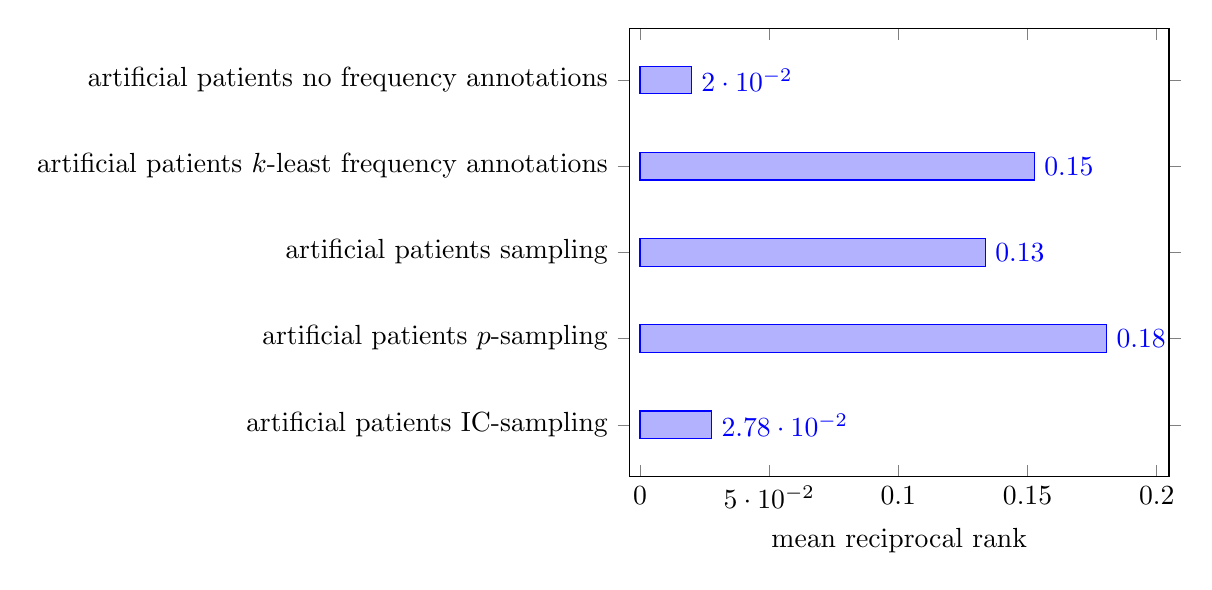
\begin{tikzpicture}
        \begin{axis}[
            xbar,
            enlargelimits=0.15,
            xlabel={mean reciprocal rank},
            symbolic y coords={
                % UPSIDE DOWN!
                artificial patients IC-sampling,
                artificial patients $p$-sampling,
                artificial patients sampling,
                artificial patients $k$-least frequency annotations,
                artificial patients no frequency annotations,
            },
            ytick=data,
            nodes near coords, 
            nodes near coords align={horizontal},
            yticklabel style={text height=1.5ex}, % To make sure the text labels are nicely aligned
            ]
            \addplot coordinates{
                (0.020012015728,artificial patients no frequency annotations)
                (0.152694351749,artificial patients $k$-least frequency annotations)
                (0.133770278138,artificial patients sampling)
                (0.180666666667,artificial patients $p$-sampling)
                (0.0277964713493,artificial patients IC-sampling)
            };
        \end{axis}
    \end{tikzpicture}
    \caption{Mean reciprocal rank plot for artificial patients, for only diseases with negative annotations.}
\end{figure}

\begin{figure}[h]
    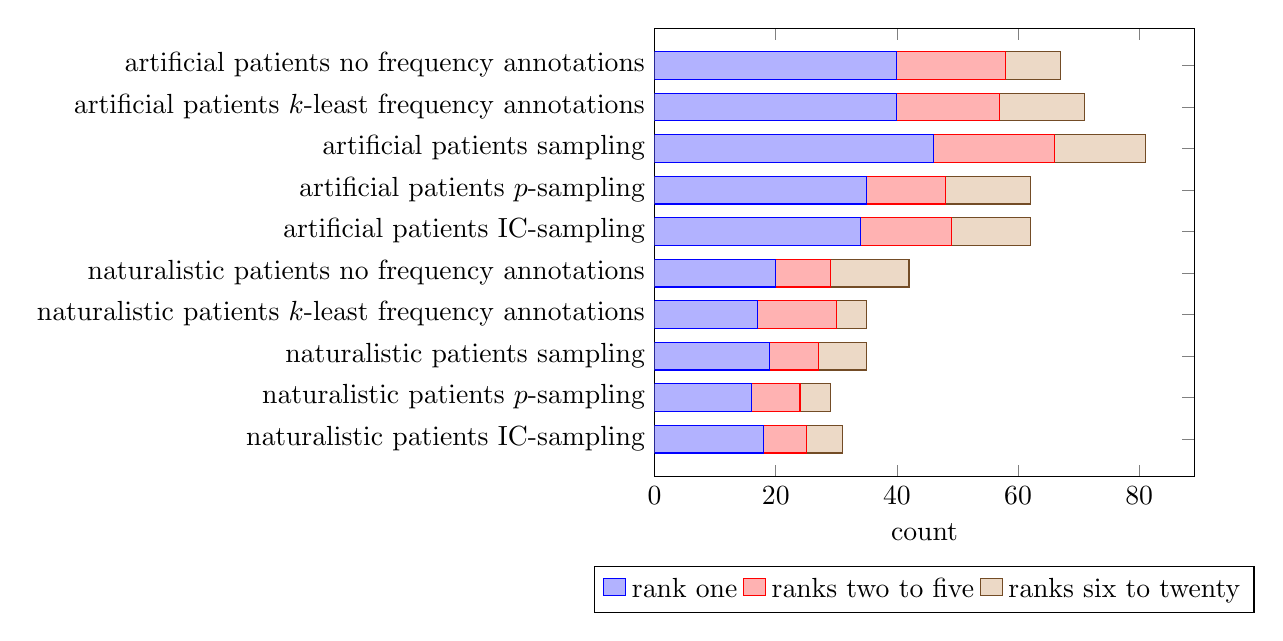
\begin{tikzpicture}
        \begin{axis}[
            xbar stacked,
            xlabel={count},
            xmin=0,
            legend style={at={(0.5,-0.20)}, anchor=north,legend columns=-1},
            symbolic y coords={
                % UPSIDE DOWN!
                naturalistic patients IC-sampling,
                naturalistic patients $p$-sampling,
                naturalistic patients sampling,
                naturalistic patients $k$-least frequency annotations,
                naturalistic patients no frequency annotations,
                artificial patients IC-sampling,
                artificial patients $p$-sampling,
                artificial patients sampling,
                artificial patients $k$-least frequency annotations,
                artificial patients no frequency annotations,
            },
            ytick=data,
            yticklabel style={text height=1.5ex}, % To make sure the text labels are nicely aligned
            ]
            \addplot coordinates{
                (40,artificial patients no frequency annotations)
                (40,artificial patients $k$-least frequency annotations)
                (46,artificial patients sampling)
                (35,artificial patients $p$-sampling)
                (34,artificial patients IC-sampling)
                (20,naturalistic patients no frequency annotations)
                (17,naturalistic patients $k$-least frequency annotations)
                (19,naturalistic patients sampling)
                (16,naturalistic patients $p$-sampling)
                (18,naturalistic patients IC-sampling)
            };
            \addlegendentry{rank one}
            \addplot coordinates{
                (18,artificial patients no frequency annotations)
                (17,artificial patients $k$-least frequency annotations)
                (20,artificial patients sampling)
                (13,artificial patients $p$-sampling)
                (15,artificial patients IC-sampling)
                (9 ,naturalistic patients no frequency annotations)
                (13,naturalistic patients $k$-least frequency annotations)
                (8 ,naturalistic patients sampling)
                (8 ,naturalistic patients $p$-sampling)
                (7 ,naturalistic patients IC-sampling)
            };
            \addlegendentry{ranks two to five}
            \addplot coordinates{
                (9 ,artificial patients no frequency annotations)
                (14,artificial patients $k$-least frequency annotations)
                (15,artificial patients sampling)
                (14,artificial patients $p$-sampling)
                (13,artificial patients IC-sampling)
                (13,naturalistic patients no frequency annotations)
                (5 ,naturalistic patients $k$-least frequency annotations)
                (8 ,naturalistic patients sampling)
                (5 ,naturalistic patients $p$-sampling)
                (6 ,naturalistic patients IC-sampling)
            };
            \addlegendentry{ranks six to twenty}
        \end{axis}
    \end{tikzpicture}
    \caption{Binned ranking plot for artificial and naturalistic patients, each with a general disease.}
\end{figure}

\begin{figure}[h]
    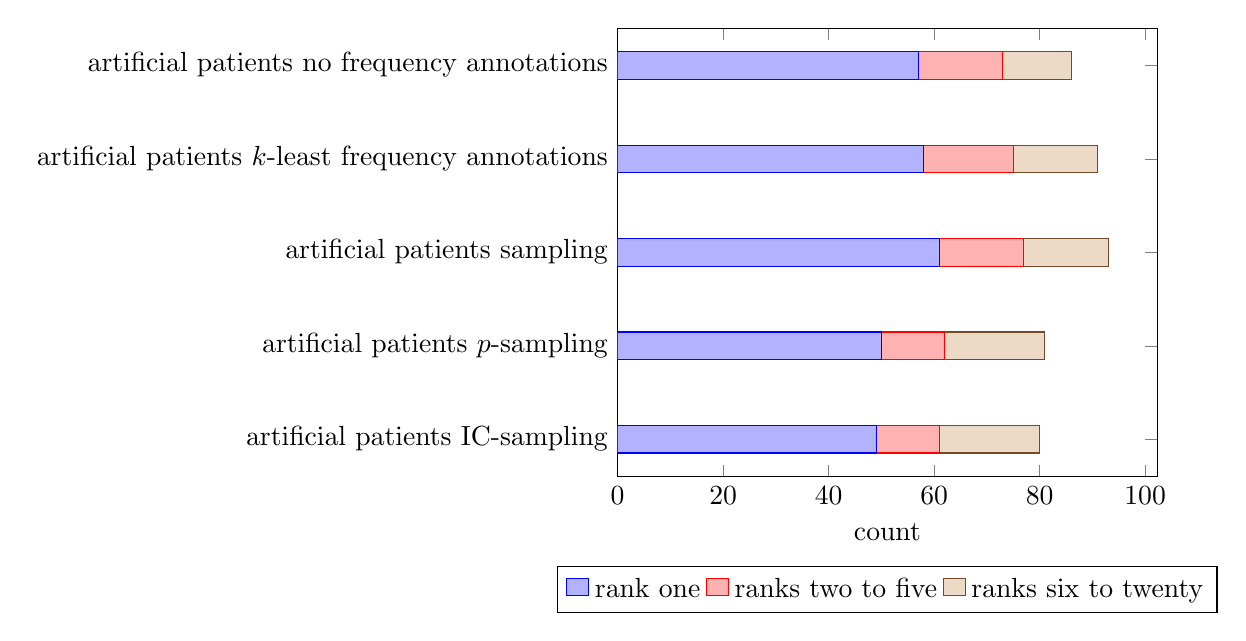
\begin{tikzpicture}
        \begin{axis}[
            xbar stacked,
            xlabel={count},
            xmin=0,
            legend style={at={(0.5,-0.20)}, anchor=north,legend columns=-1},
            symbolic y coords={
                % UPSIDE DOWN!
                artificial patients IC-sampling,
                artificial patients $p$-sampling,
                artificial patients sampling,
                artificial patients $k$-least frequency annotations,
                artificial patients no frequency annotations,
            },
            ytick=data,
            yticklabel style={text height=1.5ex}, % To make sure the text labels are nicely aligned
            ]
            \addplot coordinates{
                (57,artificial patients no frequency annotations)
                (58,artificial patients $k$-least frequency annotations)
                (61,artificial patients sampling)
                (50,artificial patients $p$-sampling)
                (49,artificial patients IC-sampling)
            };
            \addlegendentry{rank one}
            \addplot coordinates{
                (16,artificial patients no frequency annotations)
                (17,artificial patients $k$-least frequency annotations)
                (16,artificial patients sampling)
                (12,artificial patients $p$-sampling)
                (12,artificial patients IC-sampling)
            };
            \addlegendentry{ranks two to five}
            \addplot coordinates{
                (13,artificial patients no frequency annotations)
                (16,artificial patients $k$-least frequency annotations)
                (16,artificial patients sampling)
                (19,artificial patients $p$-sampling)
                (19,artificial patients IC-sampling)
            };
            \addlegendentry{ranks six to twenty}
        \end{axis}
    \end{tikzpicture}
    \caption{Binned ranking plot for artificial patients, each infected with a disease that has negative annotations.}
\end{figure}
